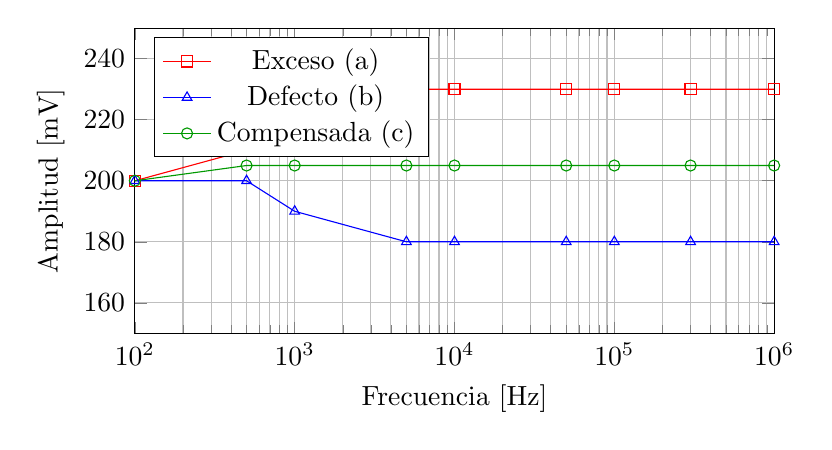
\begin{tikzpicture}
\begin{semilogxaxis}[
    width=0.8\textwidth,
    height=0.45\textwidth,
    grid=both,
    xlabel={Frecuencia [\unit{Hz}]},
    ylabel={Amplitud [\unit{mV}]},
    xmin=100, xmax=1000000,
    ymin=150, ymax=250,
    legend pos=north west,
]

% Caso (a) - Exceso de compensación
\addplot[color=red, mark=square] coordinates {
    (100, 200)
    (500, 210)
    (1000, 215)
    (5000, 230)
    (10000, 230)
    (50000, 230)
    (100000, 230)
    (300000, 230)
    (1000000, 230)
};
\addlegendentry{Exceso (a)}

% Caso (b) - Defecto de compensación
\addplot[color=blue, mark=triangle] coordinates {
    (100, 200)
    (500, 200)
    (1000, 190)
    (5000, 180)
    (10000, 180)
    (50000, 180)
    (100000, 180)
    (300000, 180)
    (1000000, 180)
};
\addlegendentry{Defecto (b)}

% Caso (c) - Compensada (Respuesta plana)
\addplot[color=green!60!black, mark=o] coordinates {
    (100, 200)
    (500, 205)
    (1000, 205)
    (5000, 205)
    (10000, 205)
    (50000, 205)
    (100000, 205)
    (300000, 205)
    (1000000, 205)
};
\addlegendentry{Compensada (c)}

\end{semilogxaxis}
\end{tikzpicture}
